\documentclass{article}
\usepackage{amsmath}
\usepackage{tikz}
\usetikzlibrary{arrows.meta}

\begin{document}

\begin{figure}[h]
    \centering
    \begin{tikzpicture}[scale=0.8]
        % Diagram 1
        \draw[thick] (0,0) -- (2,0);
        \draw[thick] (0,1) -- (2,1);
        \draw[thick] (0,2) -- (2,2);
        \draw[thick, blue] (0,3) -- (2,3);
        \draw[->, thick] (2,0) -- (4,0);
        \draw[->, thick] (2,1) -- (4,1);
        \draw[->, thick] (2,2) -- (4,2);
        \draw[->, thick, blue] (2,3) -- (4,3);
        
        % Arrow and label for Diagram 1
        \draw[->, thick] (5,1.5) -- (6,1.5);
        \node at (5.5,1.5) {Prop. 5.4};
        
        % Diagram 2
        \draw[thick] (7,0) -- (9,0);
        \draw[thick] (7,1) -- (9,1);
        \draw[thick] (7,2) -- (9,2);
        \draw[thick, blue] (7,3) -- (9,3);
        \draw[->, thick] (9,0) .. controls (8,1) and (8,2) .. (9,3);
        \draw[->, thick] (9,1) -- (11,1);
        \draw[->, thick] (9,2) -- (11,2);
        \draw[->, thick, blue] (9,3) -- (11,3);
        
        % Arrow and label for Diagram 2
        \draw[->, thick] (12,1.5) -- (13,1.5);
        \node at (12.5,1.5) {Rotate};
        
        % Diagram 3
        \draw[thick] (14,0) -- (16,0);
        \draw[thick] (14,1) -- (16,1);
        \draw[thick] (14,2) -- (16,2);
        \draw[thick, blue] (14,3) -- (16,3);
        \draw[->, thick] (16,0) -- (14,2);
        \draw[->, thick] (16,1) -- (14,1);
        \draw[->, thick] (16,2) -- (14,0);
        \draw[->, thick, blue] (16,3) -- (14,3);
        
        % Arrow and label for Diagram 3
        \draw[->, thick] (17,1.5) -- (18,1.5);
        \node at (17.5,1.5) {Reverse};
        
        % Diagram 4
        \draw[thick] (19,0) -- (21,0);
        \draw[thick] (19,1) -- (21,1);
        \draw[thick] (19,2) -- (21,2);
        \draw[thick, blue] (19,3) -- (21,3);
        \draw[->, thick] (21,0) .. controls (20,1) and (20,2) .. (21,3);
        \draw[->, thick] (21,1) -- (19,1);
        \draw[->, thick] (21,2) -- (19,2);
        \draw[->, thick, blue] (21,3) -- (19,3);
        
        % Arrow and label for Diagram 4
        \draw[->, thick] (22,1.5) -- (23,1.5);
        \node at (22.5,1.5) {Reverse};
        
        % Diagram 5
        \draw[thick] (24,0) -- (26,0);
        \draw[thick] (24,1) -- (26,1);
        \draw[thick] (24,2) -- (26,2);
        \draw[thick, blue] (24,3) -- (26,3);
        \draw[->, thick] (26,0) .. controls (25,1) and (25,2) .. (26,3);
        \draw[->, thick] (26,1) -- (24,1);
        \draw[->, thick] (26,2) -- (24,2);
        \draw[->, thick, blue] (26,3) -- (24,3);
        
        % Arrow and label for Diagram 5
        \draw[->, thick] (27,1.5) -- (28,1.5);
        \node at (27.5,1.5) {Rotate};
        
        % Diagram 6
        \draw[thick] (29,0) -- (31,0);
        \draw[thick] (29,1) -- (31,1);
        \draw[thick] (29,2) -- (31,2);
        \draw[thick, blue] (29,3) -- (31,3);
        \draw[->, thick] (31,0) -- (29,2);
        \draw[->, thick] (31,1) -- (29,1);
        \draw[->, thick] (31,2) -- (29,0);
        \draw[->, thick, blue] (31,3) -- (29,3);
        
        % Arrow and label for Diagram 6
        \draw[->, thick] (32,1.5) -- (33,1.5);
        \node at (32.5,1.5) {Reverse};
        
        % Diagram 7
        \draw[thick] (34,0) -- (36,0);
        \draw[thick] (34,1) -- (36,1);
        \draw[thick] (34,2) -- (36,2);
        \draw[thick, blue] (34,3) -- (36,3);
        \draw[->, thick] (36,0) .. controls (35,1) and (35,2) .. (36,3);
        \draw[->, thick] (36,1) -- (34,1);
        \draw[->, thick] (36,2) -- (34,2);
        \draw[->, thick, blue] (36,3) -- (34,3);
        
        % Arrow and label for Diagram 7
        \draw[->, thick] (37,1.5) -- (38,1.5);
        \node at (37.5,1.5) {Rotate};
        
        % Diagram 8
        \draw[thick] (39,0) -- (41,0);
        \draw[thick] (39,1) -- (41,1);
        \draw[thick] (39,2) -- (41,2);
        \draw[thick, blue] (39,3) -- (41,3);
        \draw[->, thick] (41,0) -- (39,2);
        \draw[->, thick] (41,1) -- (39,1);
        \draw[->, thick] (41,2) -- (39,0);
        \draw[->, thick, blue] (41,3) -- (39,3);
        
        % Arrow and label for Diagram 8
        \draw[->, thick] (42,1.5) -- (43,1.5);
        \node at (42.5,1.5) {Reverse};
    \end{tikzpicture}
    
    \caption{The saddle moves of Proposition \ref{prop:newii} are consistent under mirror image, as explained in the proof of Proposition \ref{prop:newimirror}.}
    \label{fig:saddle_moves_mirror}
\end{figure}

\end{document}